% actividades

\subsection{Calendário completo}
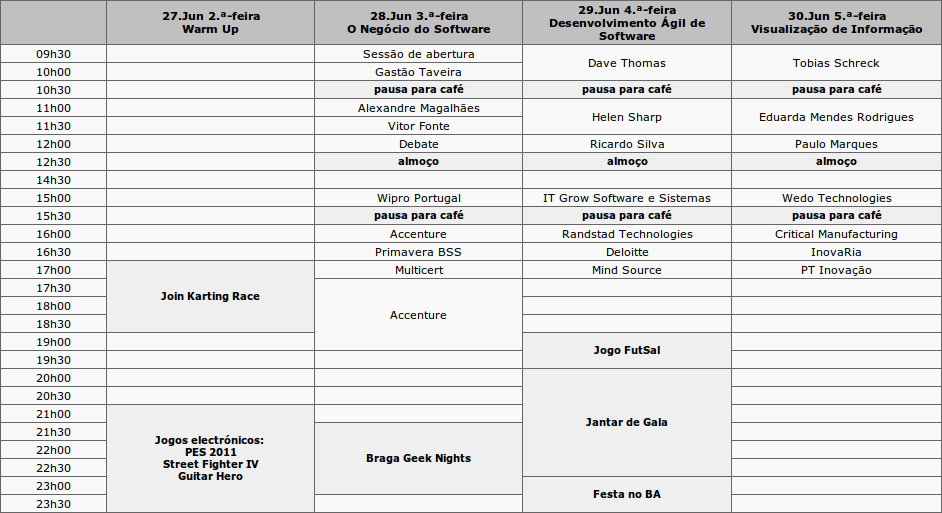
\includegraphics[width=\textwidth]{material/tabela_plano.png}

\subsection{Join Karting Race}
Prova de Karting com equipas de 4 elementos.\\
Duração: 20 min./elemento.\\
Local: Kartódromo Internacional de Braga\\
Prémio: inscrição gratuita no jantar de gala\\

\subsection{Gastão Taveira}
Tema: O negócio de Produtos de Software Empresarial (Enterprise SW)\\

O negócio de Produtos Software é complexo; não é só escrever 
código. Exige um grande cuidado na montagem de Estratégia de Produto; 
\\
Estratégia  Comercial; Metodologias; Processos (ex.Product Life 
Cycle); Organização (PD,  QA, Doc, Delivery, Tech Support – Sales, 
Pre-Sales, etc.) Há opções estratégicas de fundo para as empresas de SW. Empresas muito  diferentes, com vocações e processos muito distintos. Altitude Software optou por estratégia clara: Produto standardizado; Focalização em nicho; Mercado Global. Organização, Processos, Metodologias sintonizados com estratégia. Gastao Taveira é CEO da Altitude Software desde 2003. É um dos principais accionistas da empresa, após ter liderado um consórcio de investidores que a adquiriram e salvaram da falência nesse mesmo ano.\\

No últimos oito anos, Gastão Taveira esteve fortemente envolvido na 
área de Tecnologias de Informação, tendo estado envolvido outros 2 
projectos empresarias:\\
\begin{itemize}
\item Enabler, um integrador de sistemas baseado no Porto, de que foi accionista e Managing Director após um Management Buy Out; esta empresa viria a ser adquirida pela empresa indiana Wipro em 2005.
\item MobiComp, uma empresa de soluções de mobilidade, baseada em Braga, de que foi sócio fundador e administrador até á sua aquisição em 2008 pela Microsoft.
\end{itemize}

Quando se tornou empreendedor na área das Tecnologias de Informação, 
Gastão Taveira tinha atrás de si uma carreira de mais de 15 anos no campo da gestão internacional, tendo desempenhado funções na McKinsey \& Co (conultadoria estratégica) e no grupo Credit Suisse (serviços financeiros).<br>Gastão Taveira licenciou-se em Engenharia Civil pela Universidade do Porto em 1981 e graduou-se em Master of Business Administration (MBA) pelo INSEAD (Fontainebleau, França) em 1984.

\subsection{Alexandre Magalhães}
Tema: Alpha Male Apps

Uma viagem pelos meandros dos emergentes mercados digitais de aplicações. Partindo nos diversos modelos de negócio disponíveis e as diferenças entre as várias lojas de aplicações. Visitando os desafios que estes impõem ao nível da promoção e capacidade de monetização. E terminando nas estratégias de marketing obrigatórias para sustentar o crescimento continuo das vendas e da marca.<br>Usando vários exemplos, experiências, erros e sucessos da marca NDrive dentro das lojas de aplicações, apresentar os Do and don't deste mercado de crescimento exponencial.

Alexandre Magalhães é Director de Marketing da NDrive. Ser Director de Marketing numa empresa multinacional de tecnologia, significa antecipar o futuro e testar hoje as regras de mercado de amanhã. Viciado em ambientes de constante mudança, o Alexandre considera a NDrive como um projeto de vida. Desde as salas criativas de Budapeste, até ao emergente e dinâmico mercado das App Stores, não há limites (que não a capacidade física) para a implementação de novas ideias. Acreditando que o futuro da navegação é cada vez mais o que está para além da simples indicação de um percurso, o Alexandre visiona o NDrive como um assistente pessoal presente no bolso de cada utilizador.

\subsection{Dave Thomas}
Dave Thomas has a wide spectrum of experience in the software industry as an engineer, professor, consultant, architect, executive and investor. Dave is founder and CEO of Bedarra Corporation; which provides virtual CTO and CEO, business mentoring and seed investment to emerging companies. Recently formed Bedarra Research Labs undertakes speculative research on applications of emerging software technologies.  He has many years of experience in structured documents including the design of laser printer controllers, early commercial applications of Tex. He has advised on the IBM B2B strategy, and is on the MS Customer Advisory Council and with OLL contributed to the SCORM elearning standard, and authoring tools. He is Chairman of Xia Systems, Online-Learning.com (OLL), and a director of Stilo/Omnimark, Bitflash, Amikanow and Synop and several other software companies.  Dave is best known as the founder and past CEO and president of Object Technology International Inc. (formerly OTI, now IBM OTI Labs) and led the commercial introduction of object and component technology. The company is often cited as the ideal model of a software technology company.  He was also the principal visionary and architect for IBM VisualAge Smalltalk and Java tools and virtual machines including the initial work on popular multi-language Eclipse.org IDE. OTI pioneered the use of virtual machines in embedded systems with Tektronix shipping the first commercial products in 1988. He was instrumental in the establishment of IBM’s Pervasive computing efforts and in particular the Java tooling.  Dave is an adjunct research professor at Carleton University, and the University Of Queensland and is widely published in the software engineering literature. He is a popular humorous albeit opinionated keynote speaker. Dave remains active in various roles within the technical community including ECOOP, AOSD, Evolve, and Agile Development Conference, Agile/XP Universe and OOPSLA Onward. He is a founding director of the Agile Alliance and most recently a founder of Open Augment Consortium. Dave writes expert columns in Otland Online in Germany, and the Journal Of Object Technology in Switzerland where he also serves on the editorial board.

\subsection{Helen Sharp}
Tema: Requirements Engineering in an agile team

Agile software development promotes feedback, discipline and close collaboration between all members of the development team, and de-emphasises documentation, ‘big design up front’ dedicated analysis tools and hierarchical processes. Evidence from practice indicates that two simple physical artefacts (story cards and the wall), used in a particular and disciplined manner, and supported by appropriate social activity, are key to the success of co-located agile teams. These artefacts are the closest thing that many agile teams have to a set of requirements. However a cognitive dimensions analysis of these artefacts reveals that they are not good at showing an overview of the structure of the code, nor the functionality being offered. Instead, functional attributes and structure of the software is communicated, evolved and kept through social activities such as pairing and customer collaboration. In this talk I will provide an overview of a typical ‘day in the life’ of an XP team and discuss the team’s requirements engineering activities.

Helen Sharp is Professor of Software Engineering at the Open University, UK. Helen’s research focuses on the study of professional software practice and the effect of human and social aspects on software development. She has been conducting qualitative studies of software practice since the early 1990s, and delights in adopting techniques and theoretical frameworks from other disciplines such as distributed cognition, cognitive dimensions, and technological frames. She is very active in both the software engineering and interaction design (HCI) communities and has had a long association with practitioner-related conferences. Helen is joint author of one of the leading textbooks on Interaction Design (id-book.com); its third edition was launched at CHI 2011. She is co-editor of the Voice of Evidence column for IEEE Software, and reviews for many journals and conferences. For more information see http://mcs.open.ac.uk/hcs2

\subsection{Ricardo Silva}
Tema: Mobilidade em Ambientes de Acesso Heterogéneos com Terminais Android

O paradigma de acesso à Internet está a mudar e um novo e vasto conjunto de novas tecnologias de acesso wireless, como por exemplo WiMAX, Wi-Fi e 3GPP UMTS/LTE, estão agora ao dispor dos utilizadores e dos seus terminais multi-acesso. Deste modo, novos mecanismos e protocolos são necessários para fornecer mobilidade transparente entre todas as tecnologias de acesso mencionadas. Actualmente, o organismo de normalização IEEE, nomeadamente o grupo 802.21, está a definir uma plataforma para otimizar os processos de mobilidade em redes de acesso heterogéneas, designada Media Independent Handover (MIH) framework.  <br> Tendo como base o framework MIH definido pelo IEEE 802.21 e protocolos de mobilidade IP do IETF, este projeto propõe a definição de um conjunto de mecanismos e procedimentos com o objetivo de fornecer mobilidade transparente aos utilizadores em ambientes de acesso heterogéneos. Neste sentido, este trabalho focar-se-á na investigação e implementação da norma IEEE 802.21 em terminais móveis com o sistema operativo Android, com o intuito de assegurar a mobilidade entre redes de acesso Wi-Fi e 3G (UMTS), com níveis de qualidade e desempenho adequados.

Ricardo Silva, licenciado em Engenharia Informática pela Universidade do Minho em 2008 e com o título de Mestrado em Engenharia Informática também pela Universidade do Minho em 2010. Em 2009 entrou na PT Inovação, onde no último ano esteve a desenvolver principalmente para Android e Windows, na área de cloud computing, mobilidade heterogénea e autenticação EAP-SIM em redes Wi-Fi. Durante este tempo tem feito contribuições para projectos Europeus, como o Hurricane, Cloud4SOA, Medieval e projetos Eurescom.

\subsection{Jogo FutSal}
Actividade: jogo de Futsao.
Jogo entre alunos de lei+lcc contra professores+funcionários do DI.
Local: Pavilhão Gimnodesportivo de Gualtar.

\subsection{Jantar de Gala}
Local: restaurante do Hotel Meliã Braga

\subsection{Tobias Schreck}
Tema: Information Visualization and Visual Analytics for Understanding and Analyzing Data – Principles, Applications, and Challenges

Today, tremendous amounts of data are collected and generated in many application areas. In domains such as finance and business, engineering, science, or the mass media, large amounts of data arise. Understanding and analyzing large amounts of data is decisive for innovation and application results. However, effective access and understanding of data are often hindered by data sizes and complexities involved, and there is a danger that users get lost in an overload of information. Information Visualization is concerned with finding computer-based visual representations and interaction modalities for data such that understanding and insight are fostered. Visual Analytics is concerned with integrating the analytic capabilities of the computer and the abilities of the human analyst in designing interactive visual analysis systems. In this talk we will review important principles underlying the research areas of Information Visualization and Visual Analytics. By example techniques from different application and data domains, we will discuss how visual representations coupled with automatic analysis methods can help to understand and analyze large, complex data sets. We will also discuss open research challenges and future trends in the area.

Tobias Schreck is an Assistant Professor for Visual Analytics with the Department for Computer and Information Science at University of Konstanz, Germany. Between 2007 and 2011, he was a postdoc researcher at Technische Universitaet Darmstadt, Germany, where he headed a research group on visual search and analysis. He obtained a PhD in Computer Science in 2006, and a Master of Science degree in Information Engineering in 2002, both from University of Konstanz. Tobias Schreck works in the areas of Information Visualization, Visual Analytics, and Digital Libraries. His research interests include visual search and analysis in time-oriented, high-dimensional, and 3D object data, with applications in data analysis and multimedia retrieval. Tobias Schreck is leading a research project on visual feature space analysis, supported by the German Research Foundation DFG. He published more than 60 scientific papers, and was a co-chair of the Eurographics Workshop on 3D Object Retrieval in 2010 and 2011.

\subsection{Eduarda Mendes Rodrigues}
Tema: Visual Analytics at the Age of the Social Web

Social media services have become a global phenomenon on the Internet, enabling new forms of communication among people for nearly every purpose imaginable. The popularity of these services provides an opportunity to study the characteristics of online social networks and derive valuable knowledge from the massive amounts of user-generated content. This talk presents a process model of social network analysis and visualization, describing the key concepts and techniques for making sense of social media data. Several visualizations of social and information networks are presented to illustrate the power of visual analysis for mining online communities and user-generated content, as well as to highlight the challenges of large-scale data visualization.

Eduarda Mendes Rodrigues is an Assistant Professor at the Department of 
Informatics Engineering, Faculty of Engineering of the University of Porto, Portugal. She holds a Ph.D. in Electronic \& Electrical Engineering from University College London, UK, and a Licentiatura degree in Electrical and Computer Engineering from the University of Porto, Portugal. Eduarda's prior experience includes a 4-year post-doctoral position at Microsoft Research Cambridge, UK and a 1-year research fellow position at University College London, UK. Eduarda's research broadly covers the areas of data mining and web information retrieval, with particular emphasis on social network mining and user-centred technologies for social computing. She is currently involved in FCT-UT Austin, Microsoft External Research and QREN funded projects and is an active member of the US-based Social Media Research Foundation. Eduarda has published in top international venues and is the co-author of three US patent applications.

\subsection{Paulo Marques}
Tema: CEP 2.0: Next Generation Real-Time Data Processing

One of the toughest problems companies face today is how to make decisions that mater. Moreover, those decisions have to be made quickly and accurately, in real-time. FeedZai Pulse is a revolutionary next-generation real-time business intelligence system. Having at its core a powerful complex event processing engine, it seamlessly integrates real-time data with historical information, creating a complete platform for managing, understanding and extracting value from the huge data volumes flowing on the modern enterprises. In this presentation we will discuss the challenges associated with large-scale data processing and explore how solutions have been deployed in areas like real-time monitoring of bank transactions, real-time ETL of Call-Detail-Records for telecommunication operators, smart-grid energy monitoring for large-scale deployments, wind-farm operational performance compliance verification and Service Level Agreement (SLA) control.

Paulo Marques is the CTO of FeedZai, a Top-20 European smart company specialized in large-scale real-time business intelligence. Paulo is also an Assistant Professor at the University of Coimbra and Adjunct Associate Teaching Professor at Carnegie Mellon. Over the last years he lead and worked in a large number of projects for institutions like the European Space Agency, Microsoft Research, Critical-Software, SciSys, Siemens, Ericsson, among many others. Paulo holds a PhD from the University of Coimbra.


